\documentclass[12pt,a4paper,oneside]{book}
\usepackage[a4paper,left=20mm,right=10mm,top=10mm,bottom=10mm]{geometry}
%   bindingoffset=0mm}

\usepackage[utf8]{inputenc}
\usepackage[german,english,russian]{babel}
\usepackage[unicode]{hyperref}
% \hypersetup{unicode=true}

\usepackage{graphicx}
\usepackage{xcolor}
% \usepackage{menukeys} can't download package
\newcommand{\keys}[1]{\textbf{[#1]}}
\newcommand{\file}[1]{\textbf{#1}}

\newcommand{\DE}[1]{\textcolor{green}{#1}} 
\newcommand{\RU}[1]{\textcolor{red}{#1}}
\newcommand{\TRpart}[2]{\part{#2 /#1/}}
\newcommand{\TRchapter}[2]{\chapter{#1\\#2}}
\newcommand{\TRsection}[2]{\section{#1\\#2}}
\newcommand{\TRsubsection}[2]{\subsection{#1\\#2}}
\newcommand{\TRsubsubsection}[2]{\subsubsection{#1\\#2}}
\newcommand{\TRparagraph}[2]{\paragraph{#1\\#2\\}}



\title{Стойка ЧПУ KOSY и NCCAD7}
\author{перевод Dmitry Ponyatov <dponyatov@gmail.com>}

\begin{document}

\maketitle

\RU{Кривой перевод оригинальной документации из поставки учебного комплекта станков
WABECO~--- файлы \file{nccad7.chm} и \file{ZSE3Help.chm} с немецкого.
Комплектность поставки документации от ecoinvent хромает, могли бы хотя бы
английский вариант положить как опцию.}

\tableofcontents

\DE{Hilfethemen für nccad7 - 18. 02. 2005}
\RU{Справка для nccad7 - 18 02, 2005}
\DE{Überarbeitet: August 2002}
\RU{Редакция: Август 2002}

\TRpart{NCCAD7}{NCCAD7}

\TRchapter{Suchen von Worten}{Поиск по словам}

\bigskip 

\DE{Angenommen Sie möchten eine nähere Erklärung zum Begriff "Nullpunkt".}
\RU{Вероятно Вы хотели бы более точное определение термина
"нулевая точка".}
\DE{Innerhalb aller Hilfethemen kommt dieser Begriff auf mehreren Seiten vor.}
\RU{Кажется что этот термин используется на каждой странице этого
документа.}
\DE{Um diese Seiten - und die zugehörigen Textstellen zu finden gibt es die
Funktion "Suchen".}
\RU{Чтобы найти такие страницы и соответствующие места в тексте,
существует функция ``Поиск''}
\DE{Sie gehen folgendermaßen vor:}
\RU{Он используется следующим образом:}
\begin{enumerate}
  \item Öffnen Sie die Karteikarte \textbf{Suchen} durch Klick auf den Reiter
  "Suchen".
  \item Geben Sie im \textbf{Feld Suchbegriff} das Suchwort komplett ein. 
\begin{enumerate}
  \item Achten Sie auf Rechtschreibung. 
  \item Die Klein/Großschreibung wird in der Suchfunktion nicht beachtet, z.B.
  \item kann eingegeben werden "nullpunkt" oder "Nullpunkt".
  \item Schon einmal eingegebene Suchworte sind über das PullDown-Menü wieder
  aufrufbar (Pfeil nach unten).
  \item In den Suchbegriff können logische Verknüpfungen eingebaut werden, die
Sie über den Button "Pfeil nach rechts" neben dem Eingabefeld erreichen.
\end{enumerate}
  \item Klicken Sie auf "Themen auflisten". Eine Liste mit den Seiten, in denen
das Suchwort mindestens einmal vorkommt, erscheint.
  \item Wählen Sie durch Doppelklick eine dieser Seiten aus. In der
dargestellten Seite werden die gefundenen Textstellen markiert. Durch Scrollen können
 Sie die Textstellen auffinden. (Siehe Bild, unterer Teil).
\end{enumerate}

\bigskip

Das folgende Bild gibt einen Überblick über die verschiedenen Phasen des Suchens:

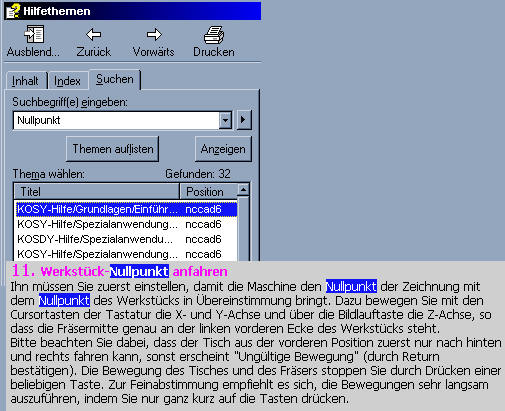
\includegraphics{pic/Suche1.png}

\TRchapter{Das Indexregister}{Индексный регистр}

\DE{Falls Sie mehr Informationen über einen bestimmten Themenbereich oder über
eine bestimmte Anwendung haben möchten, finden Sie im Indexregister alle
erdenklichen Stichworte.}
\RU{Если бы Вы хотели иметь большую информацию об определенной теме или
применении, вы можете найти в разделе ``Индекс'' возможные ключевые слова.}
\DE{Diese Stichworte sind nach Themenbereichen
gegliedert.}
\RU{Ключевые слова разделены на тематические области.}

\bigskip

\textbf{Bedienung des Indexregisters}

\bigskip

Geben Sie den Begriff in das Feld "Zu suchendes Schlüsselwort"\ ein. 
Nach jedem
eingegebenen Buchstaben werden Sie im Indexfenster weitergeleitet:

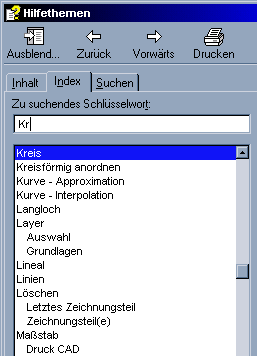
\includegraphics{pic/Suche2.png}

Wenn Sie den richtigen Begriff gefunden haben klicken Sie ihn doppelt an. Im rechten Fenster 
erscheint die Hilfsseite, die das Thema erläutert.

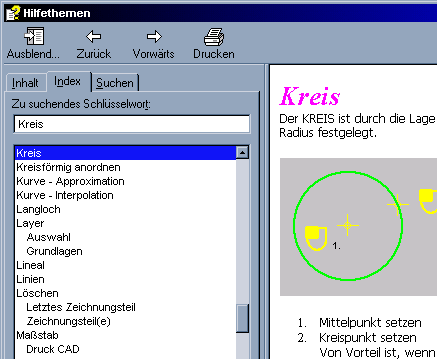
\includegraphics{pic/Suche3.png}

\TRchapter{Grundlagen der Bedienung}{Основные принципы работы}
	\TRsection{Kurzanleitung}{Краткое руководство}
	\TRsection{Bedienprinzip}{Принцип действия}
	\TRsection{Drucken}{Печать}
	\TRsection{Konfiguration von nccad7}{Конфигурирование nccad7}
	\TRsection{Vorlagen}{Шаблоны}
	\TRsection{Das Menü}{Меню}
		\TRsubsection{Ansicht}{Вид}
		\TRsubsection{Datei}{Файл}
		\TRsubsection{Hilfe}{Помощь}
		\TRsubsection{Maschine}{Станок}
		\TRsubsection{Parameter}{Параметры}
		\TRsubsection{Simulation}{Симуляция}
		
	\TRsection{Die Icons}{Иконки}
		\TRsubsection{Bearbeitung}{Обработка}
			\TRsubsubsection{Drehen}{Стрелять}
			\TRsubsubsection{Eigenschaften ändern}{Изменение свойств}
			\TRsubsubsection{Konstruktionspunkt verschieben}{Перемещение узлов}
			\TRsubsubsection{Kopieren}{Копировать}
			\TRsubsubsection{Korrektur Texte}{Исправление текста}
			\TRsubsubsection{Kreisförmig anordnen}{Круговое выравнивание}
			\TRsubsubsection{Löschen}{Удалить}
			\TRsubsubsection{Löschen Letztes}{Удалить последнюю}
			\TRsubsubsection{Rückgängig Letztes}{Отменить последнее}
			\TRsubsubsection{Skalieren}{Масштабирование}
			\TRsubsubsection{Spiegeln horizontal}{Отразить горизонтально}
			\TRsubsubsection{Spiegeln horizontal mit Kopie}{Отразить горизонтально с
			копией}
			\TRsubsubsection{Spiegeln vertikal}{Зеркалить вертикально}
			\TRsubsubsection{Spiegeln vertikal mit Kopie}{Зеркалить вертикально с копией}
			\TRsubsubsection{Verschieben}{Сдвинуть}
			\TRsubsubsection{Zoom Maßstab}{Зум}
			
		\TRsubsection{CAD - 3D}{}
			\TRsubsubsection{Ansicht dreidimensional}{Трехмерное изображение}
			\TRsubsubsection{Plastische Zone Kreis}{Пластичная зона Круг}
			\TRsubsubsection{Plastische Zone Rechteck}{Пластичная зона Прямоугольник}
			\TRsubsubsection{Plastische Zone in STL wandeln}{Пластичная зона Прямоугольник}
			\TRsubsubsection{Schnitt bearbeiten}{Править секцию}
			\TRsubsubsection{Schnitt neu}{Новая секция}
			
		\TRsubsection{CAD - Besonderes}{CAD - Фичи}
			\TRsubsubsection{Ellipse}{Эллипс}
			\TRsubsubsection{Freihand}{От руки}
			\TRsubsubsection{Kurve Approximation}{Аппроксимация кривых}
			\TRsubsubsection{Kurve Interpolation}{Интерполяция кривых}
			\TRsubsubsection{Mathematische Funktion}{Математические функции}
			\TRsubsubsection{Outline - Generierung}{Outline - генерация}
			\TRsubsubsection{Pad/Bahn - Generierung}{Pad/Bahn - генерация}
			\TRsubsubsection{Schraffieren}{Колодец}
			\TRsubsubsection{Tangente}{Касание}
			\TRsubsubsection{Tangente außen}{Внешнее касание}
			\TRsubsubsection{Tangente innen}{Внутреннее касание}
			\TRsubsubsection{Zahnrad außenverzahnt}{Внешнее зубчатое колесо}
			\TRsubsubsection{Zahnrad innenverzahnt}{Внутреннее зубчатое колесо}
			\TRsubsubsection{Zahnstange}{Зубчатая рейка}
			
		\TRsubsection{CAD - Standard}{CAD - Стандартный}
			\TRsubsubsection{Bogen}{Дуга}
			\TRsubsubsection{Gerade}{Прямая}
			\TRsubsubsection{Gravurtext MAX/einzeilig}{Гравировка MAX/однострочная}
			\TRsubsubsection{Gravurtext MAX/mehrzeilig}{Гравировка MAX/многострочная}
			\TRsubsubsection{Gravurtext TrueType}{Гравировка TrueType}
			\TRsubsubsection{Kreis}{Круг}
			\TRsubsubsection{Langloch}{Паз}
			\TRsubsubsection{Polygon}{Многоугольник}
			\TRsubsubsection{Polygon-Generierung}{Полигон генерация}
			\TRsubsubsection{Punkt}{Точка}
			\TRsubsubsection{Rechteck}{Прямоугольник}
			
 		\TRsubsection{CAM - Standard}{CAM - Стандарт}
 			\TRsubsubsection{Ausspannposition}{Позиция зажима}
 			\TRsubsubsection{Bahnkorrektur}{Коррекция трассы}
 			\TRsubsubsection{Insel auflösen}{Растворение острова}
 			\TRsubsubsection{Insel zuweisen}{Назначить Остров}
 			\TRsubsubsection{Kontur auflösen}{Растворить контур}
 			\TRsubsubsection{Kontur generieren}{Создание контура}
 			\TRsubsubsection{Leitkontur}{Ограничивающий контур}
 			\TRsubsubsection{Tasche fräsen}{Фрезерование кармана}
 			\TRsubsubsection{Technologie}{Технология}
 			\TRsubsubsection{Werkstück - Befestigung}{Заготовка - фиксация}
 			\TRsubsubsection{Werkstück - Nullpunkt}{Заготовка - Нулевая точка}
 			
 		\TRsubsection{Darstellung}{Представление}
			\TRsubsubsection{Ansicht Letzte}{Последний вид}
			\TRsubsubsection{Ausschnitt verschieben}{Переместить раздел}
			\TRsubsubsection{Ausschnitt wählen}{Выбрать раздел}
			\TRsubsubsection{Neu darstellen}{Новый вид}
			\TRsubsubsection{Tischdarstellung}{Изображение стола}
			
		\TRsubsection{Dokumentation}{Документация}
			\TRsubsubsection{Bemaßung horizontal}{Горизонтальный размер}
			\TRsubsubsection{Bemaßung Radius}{Радиусный размер}
			\TRsubsubsection{Bemaßung schräg}{Косой размер}
			\TRsubsubsection{Bemaßung vertikal}{Вертикальный размер}
			\TRsubsubsection{Bemaßung Winkel}{Угловой размер}
			\TRsubsubsection{Beschriftung TrueType}{Надпись TrueType}
			\TRsubsubsection{Beschriftung MAX/einzeilig}{Надпись MAX/однострочный}
			\TRsubsubsection{Beschriftung MAX/mehrzeilig}{Надпись MAX/многострочный}
			\TRsubsubsection{Bearbeiter}{Редактор}
			\TRsubsubsection{Bearbeiter letzte Änderung}{Редактор последнего изменения}
			\TRsubsubsection{Dateiname}{Имя файла}
			\TRsubsubsection{Datum letzte Änderung}{Дата последнего изменения}
			\TRsubsubsection{Datum aktuell}{Текущая дата}
			\TRsubsubsection{Datum Ausdruck}{Дата выражение}
			\TRsubsubsection{Datum erstellt}{Дата создания}
		\TRsubsection{Einstellungen}{Настройки}
			\TRsubsubsection{Bezugspunkt}{Контрольная точка}
			\TRsubsubsection{Fang}{Привязка}
 			\TRsubsubsection{Layer (Zeichnungslage)}{Слой (рисунок расположения)}
			\TRsubsubsection{Lineal}{Линейка}
			\TRsubsubsection{Linien}{Вектор}
			\TRsubsubsection{Raster}{Растр}
			
		\TRsubsection{Information}{Информация}
			\TRsubsubsection{Messen}{Измерение} 
			\TRsubsubsection{Zeichnungsteil-Informationen}{Рисование часть информации} 
			
 		\TRsubsection{Symbole}{Символы}
			\TRsubsubsection{Symbol auflösen}{Разрешенные символы}
			\TRsubsubsection{Symbol laden}{Загрузка символа}
			\TRsubsubsection{Symbol speichern}{Сохранение символа}
			
 		\TRsubsection{Umwandlung}{Преобразование}		
 			\TRsubsubsection{Trimmen}{Обрезка} 
			\TRsubsubsection{Verlängern}{Удлинение}
			\TRsubsubsection{Trimmen-Verlängern}{Обрезка-Удлинение}
			\TRsubsubsection{Trimmen 2 Teile}{Обрезка 2 детали}
			\TRsubsubsection{Verlängern 2 Teile}{Удлинение 2 детали}
			\TRsubsubsection{Auftrennen}{Разделение}
			\TRsubsubsection{Autom. Trimmen-Verl. (Kontur verfolgen)}{Автоматическая
			обрезка-удлинение (verfolgen трека)}
			\TRsubsubsection{Verdünnen}{Разбавление}
			\TRsubsubsection{Polygon-Generierung}{Полигон генерация}
			\TRsubsubsection{Konvertieren in Gerade}{Преобразовать в отрезки}
			\TRsubsubsection{Konvertieren in Polygon}{Преобразовать в многоугольник}
			\TRsubsubsection{Runden}{Скругление}
			\TRsubsubsection{Runden selektiv}{Селективное скругление}
			\TRsubsubsection{Fasen}{Фаска}
			\TRsubsubsection{Fasen selektiv}{Селективная фаска}

\documentclass[12pt,a4paper,oneside]{book}
\usepackage[a4paper,left=20mm,right=10mm,top=10mm,bottom=10mm]{geometry}
%   bindingoffset=0mm}

\usepackage[utf8]{inputenc}
\usepackage[german,english,russian]{babel}
\usepackage[unicode]{hyperref}
% \hypersetup{unicode=true}

\usepackage{graphicx}
\usepackage{xcolor}
% \usepackage{menukeys} can't download package
\newcommand{\keys}[1]{\textbf{[#1]}}
\newcommand{\file}[1]{\textbf{#1}}

\newcommand{\DE}[1]{\textcolor{green}{#1}} 
\newcommand{\RU}[1]{\textcolor{red}{#1}}
\newcommand{\TRpart}[2]{\part{#2 /#1/}}
\newcommand{\TRchapter}[2]{\chapter{#1\\#2}}
\newcommand{\TRsection}[2]{\section{#1\\#2}}
\newcommand{\TRsubsection}[2]{\subsection{#1\\#2}}
\newcommand{\TRsubsubsection}[2]{\subsubsection{#1\\#2}}
\newcommand{\TRparagraph}[2]{\paragraph{#1\\#2\\}}



\title{NCCAD7: Основы САПР}
\author{перевод Dmitry Ponyatov <dponyatov@gmail.com>}

\begin{document}

\maketitle
\tableofcontents
\bigskip

\TRparagraph{Grundlagen CAD}{Основы САПР}
\TRparagraph{CAD - Konstruktionsgrundlagen}{САПР - Основы дизайна}
\TRparagraph{Allgemeines}{Общая информация}

\DE{Um ein CAD-Programm zu verstehen, muß man sich zunächst mit dem
Bedienprinzip auseinandersetzen.}
\RU{Чтобы понять САПР-программу, нужно сначала разобраться с принципами работы.}
\DE{Es gibt beim Vergleich der verschiedenen
CAD-Programme zwangsläufig Gemeinsamkeiten, wie beispielsweise die Tatsache,
daß geometrische
Grundfiguren ausgewählt werden müssen.}
\RU{Сравнивая различные САПР, многие черты должны быть общими, например, тот
факт, что геометрические примитивы должны быть выбраны.}
\DE{Es gibt aber auch Unterschiede, wie
beispielsweise die Belegung der rechten Maustaste.}
\RU{Но есть и отличия, например, назначение правой кнопки мыши.}
\DE{Sie sollten deshalb die folgenden Punkte durcharbeiten und in der praktischen
Arbeit dieses Wissen anwenden.}
\RU{Таким образом, вы должны работать используя описанные далее приемы, и
применять эти знания в практической работе.}
\DE{Entweder Sie gehen in der Reihenfolge der Nummerierung alle Punkte durch
oder Sie klicken auf eines der Themen im folgenden Inhaltsverzeichnis, um zur
gewünschten Erklärung zu kommen.}
\RU{Либо вы идете в порядке нумерации всех терминов или нажмите на одну из тем в
следующей таблице содержания, чтобы получить требуемое.}
\DE{Zum Inhaltsverzeichnis kehren Sie immer wieder zurück, wenn Sie in eines der
Felder [Zurück] - oder im Browser-Menü den Button "Zurück" klicken.}
\RU{Чтобы вернуться к содержанию, если вы находитесь в одном из полей
\keys{назад} - кнопка \keys{Назад} или нажмите в меню обозревателя.}

% \TRsubsection{Inhaltsverzeichnis der Themen}{Индекс темы}

\TRchapter{Start}{Начало}

\includegraphics{pic/Kons1.png}\bigskip

\DE{Zunächst müssen Sie im Menü Datei entscheiden, ob Sie mit CNC oder CAD arbeiten
wollen, eine neue Datei erstellen- oder eine vorhandene laden wollen.}
\RU{Во-первых, вы должны решить выбрав в меню Файл, хотите ли вы работать с ЧПУ
или САПР, создать новый файл или загрузить существующий.}
\DE{Bei CNC
gelangen Sie in den Texteditor, um CNC-Programme erstellen, bearbeiten oder
ausführen zu können.}
\RU{В режиме ЧПУ откроется текстовый редактор для создания программы ЧПУ, чтобы
редактировать ее, с возможностью выполнения.}
\DE{Bei CAD starten Sie ein spezielles Konstruktionsprogramm
mit optimaler Verbindung zur CNC-Maschine.}
\RU{При выборе режима САПР запускается программа конструирования, с оптимальной
адаптацией для использования совместно со ЧПУ-станком.}
\DE{Um eine neue Zeichnung konstruieren zu können klicken Sie auf \keys{CAD/CAM
- Neue Zeichnung}.}
\RU{Для того чтобы построить новый чертеж, нажмите на \keys{CAD / CAM - новый
рисунок}.}

\TRchapter{Der CAD-Bildschirm}{Экран САПР}

\includegraphics{pic/Kons2.png}\bigskip

\DE{Sobald Sie im Menü \keys{Datei}/\keys{CAD/CAM - Neue Zeichnung} gewählt
haben, können Sie im Zeichenfeld konstruieren.}
\RU{После того как вы выбрали в меню \keys{Файл}/\keys{CAD/CAM Новый рисунок},
можно построить характер поля.}
\DE{Im Bild oben wird Ihnen die Bedeutung der
einzelnen Bereiche des CAD-Bildschirms erklärt.}
\RU{На картинке выше вы видите несколько важных областей экрана САПР.}
\DE{Links neben dem Zeichenfeld ist das ICON-Menü.}
\RU{В левой части области рисования расположено иконное меню.}
\DE{In ihm können die wichtigsten Funktionen direkt gewählt werden.}
\RU{Наиболее важные функции могут быть выбраны непосредственно в нем.}

\TRsection{Bereiche der ICON-Hauptleiste}{Области основной
    панели инструментов}

Иконное меню разделено сверху вниз на разные группы:

\begin{itemize}
  \item
\DE{Der Technologie-Bereich, der den Zugang zu den CAM- (Bearbeitungs-)
Funktionen eröffnet.}\\
\RU{Область технологий, открываеющая доступ к CAM-функциям обработки.}
  \item
\DE{Der Einstell- und Darstellungsbereich für die die Auswahl der Layer, Linien
usw. - und für die Behandlung des Zeichnungs-Ausschnittes.}\\
\RU{Область установки и отображения для выбора слоя, линии, и т.д. - а также для
лечения подписки вырез.}
  \item
\DE{Der Korrekturbereich zum Bearbeiten (editieren) von Zeichnungsteilen. }\\
\RU{Редактирование областей компенсации для обработки деталей согласно чертежа.}
  \item
\DE{Der 2D-Bereich für die Konstruktion von Zeichnungsteilen in der 
X-Y-Ebene.}\\
\RU{2D области для проектирования элементов чертежа в плоскости XY.}
  \item
\DE{Der 3D-Bereich für die Konstruktion von "Plastischen Zonen". }\\
\RU{3D область для задания "пластических зон".}
  \item
\DE{Der Dokumentations- und Informationsbereich }\\
\RU{Область документирования и информации}
\end{itemize}

\DE{Bewegen Sie zum Kennenlernen der Funktionen die Maus vom Zeichenfeld zum
ICON-Menü und dort zu einem beliebigen ICON (beispielsweise zu Gerade im 2D-Bereich),
warten Sie einen Augenblick.}
\RU{Переместите указатель мыши на любой значок в иконном меню, чтобы узнать
о его функции (например в 2D области), подождите пару секунд.}
\DE{Es erscheint ein Erklärungsfeld (ToolTip) mit der
Bedeutung dieses ICONs.}
\RU{Вы увидите всплывающее поле подсказки с функцией этой иконки.}

\TRsection{Die Status-Zeile}{Строка состояния}

\includegraphics{pic/Kons3.png}\bigskip

\DE{Sie hat eine besondere Aufgabe:}
\RU{Она имеет конкретную задачу:}
\DE{Dort "sagt" Ihnen nccad, welche Bedienschritte erwartet werden (z.B.:
Startpunkt einer Geraden wählen). }
\RU{В ней NCCAD "говорит" Вам какая операция будет выполнена (например,
выбор начальной точки линии).}
\DE{Alle zu konstruierenden Zeichnungsteile basieren auf mathematischer
Grundlage, d.h.
es müssen Koordinatenpunkte angegeben werden, mit deren Hilfe die geometrischen
Figuren berechnet - und dargestellt werden können.}
\RU{Все элементы строятся на математической основе, то есть должны быть указаны
координаты, с помощью которых рассчитываются геометрические фигуры - и могут быть отображены.}
\DE{Zunächst ist kein Zeichnungsteil vorgeschlagen, wählen Sie z.B in der}
\RU{Во-первых, ни одна часть чертежа не предлагается выбрать для}
\DE{ICON-Gruppe}
\RU{в группе иконок}
\DE{\keys{CAD Standard}}
\DE{das ICON GERADE.}
\RU{в панели иконок.} 
\DE{Sie benötigt zwei Punkte (Startpunkt und Endpunkt), die durch 2 Mausklicks (kurzes
Drücken der linken Maustaste) an 2 verschiedenen Stellen des Zeichenfeldes mit dem
 Fadenkreuz positioniert werden.}
\RU{Вам нужно указать две точки (начальная точка и конечная точка) сделав 2
щелчка (нажатием левой кнопки мыши), которые будут проставлены в двух разных 
местах рабочей области, указанных символом перекрестия.} 
\DE{Grundsätzlich wird in der Statuszeile angezeigt,
 welcher Konstruktionspunkt momentan eingegeben werden muß.}
\RU{Принцип указывается в строке состояния, в момент ввода конструкционной
точки.}

\TRchapter{CAD-Funktionswahl}{Функции выбора САПР}

\includegraphics{pic/Kons4.png}\bigskip

\TRchapter{Koordinaten beim Konstruieren}{Координаты в конструировании}

\includegraphics{pic/Kons5.png}\bigskip

    \TRsection{Möglichkeiten der Koordinaten-Angabe}{Cпособы
    задания координат}
    \TRsection{Konstruktionsbeispiel}{Пример расчета}
    \TRsection{Die Möglichkeiten der Koordinaten-Eingabe}{Возможности 
    входных координат}

\TRchapter{Ausschnitte und Darstellungsformen}{Разделы и формы}

\includegraphics{pic/Kons6.png}\bigskip

    \TRsection{Unmittelbar Veränderung der Darstellung}{Немедленно
    смените представление}
    \TRsection{ICONS für die Wahl der Darstellungsformen}{Иконки
    для выбора форматов отображения}
    \TRsection{Fang}{Привязка}

\TRchapter{Besondere Konstruktionshilfen}{Особый дизайн СПИДом}

    \TRsection{Maus fixieren (Orthogonales Zeichnen)}{Мышь Fix
    (ортогонального рисования)}
    \TRsection{Fang von Konstruktionspunkten mit dem Suchfenster}{Строительство
    ловить точки с окном поиска}
    \TRsection{Fang von deckungsgleichen Konstruktionspunkten}{привлекательным
    дизайном конгруэнтным пунктов}
    \TRsection{Gruppenbildung}{Группировка}
    \TRsection{Tastaturbelegung}{Макет}

\TRchapter{Layer (Zeichnungslagen)}{Слой (материалы для рисования)}

    \TRsection{Layer für Zeichnungs- und Frästeile}{Слои для рисования и
    фрезерной частей}
    \TRsection{Besondere Layer}{Специальный слой}

% 	\TRsection{CAD - Kurzanleitung}{CAD - краткое руководство}
% 	\TRsection{CAD - 3D Funktionen}{CAD - 3D-функции}
% 	\TRsection{CAD - Technisches Zeichnen}{CAD - Технический рисунок}
% 		\TRsubsection{Dreiseiten-Darstellung}{Три-представление}
% 		\TRsubsection{Räumliche Darstellung}{Пространственное представление}
% 		\TRsubsection{Arbeiten mit Symbolen}{Работа с символами}
% 	\TRsection{Grafik}{Графика}
% 		\TRsubsection{Bilder importieren}{Импорт изображений}
% 		\TRsubsection{Formulare}{Формы}

\end{document}



% 
% \TRchapter{CNC-Fräsmaschinen}{Фрезерные станки с ЧПУ}
% 	\TRsection{Inbetriebnahme, Erste Schritte}{Ввод в эксплуатацию, Приступая к
% работе}
%  	\TRsection{Handsteuerung}{Ручное управление}
% 	\TRsection{CNC-Fräsen}{ЧПУ Фрезеровка}
% 	\TRsection{Teach In - Programmierung}{Teach In - Программирование}
% 	\TRsection{Simulation mit OpenGL}{Моделирование в OpenGL}
% 	\TRsection{Werkzeug-Korrektur}{Коррекция инструмента}
% 	\TRsection{CAD/CAM-Fräsen}{CAD / CAM фрезерные}
% 		\TRsubsection{Einführungsbeispiel, Prinzip}{Введение, принцип}
% 		\TRsubsection{Technologie-Angaben}{Информационные технологии}
% 	\TRsection{3D-Fräsen}{3D фрезеровка}
% 		\TRsubsection{Körper aus Rippen und Spanten}{Körper aus Rippen und Spanten}
% 		\TRsubsection{Plastische Zonen}{Пластические зоны}
% 		\TRsubsection{Randzonen}{Краевые зоны}
% 		\TRsubsection{STL Grundlagen}{STL основы}
% 		\TRsubsection{STL Ebenenbearbeitung}{STL Редактирование слоев}
% 		\TRsubsection{STL 4-Achs-Bearbeitung}{STL 4-осевая обработка}
% 	\TRsection{Bearbeitungseinheiten}{Блоки обработки}
% 		\TRsubsection{Universal (Metabo)}{Universal (Metabo)}
% 		\TRsubsection{Schnellfrequenz}{Высокая частота}
% 		\TRsubsection{Drehstrom}{Фаза}
% 	\TRsection{Arbeitshinweise}{Рабочие инструкции}
% 		\TRsubsection{WNP verschieben}{Переместить WNP}
% 		\TRsubsection{Maschine aufrüsten}{Обновление машины}
% 	\TRsection{Hilfsmittel}{СПИД}
% 		\TRsubsection{Pratze, Treppenbock}{Прижим, лестничный блок}
% 		\TRsubsection{Anschlagwinkel}{Параллельки}
% 	\TRsection{Spezialanwendungen}{Специальные применения}
% 		\TRsubsection{Mit Sonderwerkzeugen}{Использование специальных инструментов}
% 			\TRsubsubsection{Gewindefräser ZBGF}{Gewindefräser ZBGF}
% 		\TRsubsection{Gravuren}{Гравировка}
% 			\TRsubsubsection{MAX-Schriften}{MAX-шрифты}
% 			\TRsubsubsection{TrueType-Schriften}{TrueType шрифты}
% 			\TRsubsubsection{Fortlaufende Zahlen}{Нумерация}
% 			\TRsubsubsection{am Bogen}{на носу}
% 		\TRsubsection{Leiterplatten}{Печатная плата}
% 			\TRsubsubsection{Mit nccad entwerfen und fräsen}{сверление и фрезеровка с
% 			nccad}
% 			\TRsubsubsection{Von Layout-Programmen bearbeiten}{Импорт из программы
% 			разводки}
% 			\TRsubsubsection{Von Layout-Programmen bohren}{Сверление из программы
% 			разводки}
% 		\TRsubsection{Zahnräder}{Шестеренки}
% 			\TRsubsubsection{Grundlagen}{Основы}
% 			\TRsubsubsection{Bearbeiten}{Изготовление}
% 			\TRsubsubsection{Praxis}{Практика}
% 		\TRsubsection{Schneiden}{Резка}
% 			\TRsubsubsection{Schleppmesser}{Поворотный нож}
% 
% \TRchapter{CNC-Bohrmaschinen}{Расточной станок с ЧПУ}
% 	\TRsection{Bediengrundlagen}{Основная операция}
% 
% \TRchapter{CNC-Drehmaschinen}{Токарный станок с ЧПУ}
% 	\TRsection{Daten und Fakten}{Цифры и факты}
% 	\TRsection{Inbetriebnahme, Erste Schritte}{Ввод в эксплуатацию, Приступая к
% 	работе}
% 	\TRsection{CNC-Drehen}{ЧПУ точение}
% 	\TRsection{Simulation mit OpenGL}{Симуляция в OpenGL}
% 	\TRsection{Werkzeugverwaltung}{Управление инструментами}
% 	\TRsection{Testhilfen}{Средства тестирования}
% 	\TRsection{CAD/CAM-Drehen}{Токарный CAD/CAM}
% 		\TRsubsection{Prinzip}{Принцип}
% 		\TRsubsection{Mehrfachzyklen}{Несколько циклов}
% 	\TRsection{Spezialanwendungen}{Специальные применения}
% 		\TRsubsection{Gewinde-Drehen}{Нарезание резьбы}
% 		\TRsubsection{CNC-Zyklen}{CNC-Zyklen}
% 
% \TRchapter{Dosier-Systeme}{Системы дозирования}
% 	\TRsection{Grundlagen}{Основы}
% 	\TRsection{Schubdosierung}{Повысить дозу}
% 
% \TRchapter{Automatisierungs-Systeme}{Системы автоматизации}
% 	\TRsection{Grundlagen}{Основы}
% 	\TRsection{Schaltfunktionen während Bewegung}{Функции переключения во время
% 	тренировки}
% 
% \TRchapter{KOSY-Steuerungen}{Стойка KOSY}
% 	\TRsection{Standard-Ausführung}{Стандартная версия}
% 	\TRsection{Wabeco-Ausführung}{Wabeco версия}
% 
% \TRchapter{Spezial-Funktionen/Programme}{Спецфункции/программы}
% 	\TRsection{Hilfsprogramme}{Программа помощи}
% 		\TRsubsection{Zeichensatz-Editor}{Редактор шрифтов}
% 
% \TRchapter{Import/Export}{Импорт / экспорт}
% 	\TRsection{CNC-Programmexport}{Экспорт Программы ЧПУ}
% 	\TRsection{Postprozessoranpassung}{Постпроцессор}
% 	\TRsection{Schnittstellen}{Интерфейсы}
% 	\TRsection{2D-Import}{Импорт 2D}
% 		\TRsubsection{DXF}{DXF}
% 		\TRsubsection{HPGL}{HPGL}
% 		\TRsubsection{Nachbearbeitung}{Пост}
% 		\TRsubsection{Scannen und Vektorisieren}{Сканирование и векторизация}
% 	\TRsection{3D-Import}{Импорт 3D}
% 		\TRsubsection{STL}{STL}
% 	\TRsection{3D-Export}{3D экспорт}
% 		\TRsubsection{STL}{STL}
% 
% \TRchapter{Optionen und deren Bedienung}{Функции и их использование}
% 	\TRsection{Abtasten}{Отбор проб}
% 	\TRsection{Drehen}{Drehen}
% 	\TRsection{KOSY Wagen}{Корзина KOSY}
% 	\TRsection{Mindermengendosierung}{Микродозирование}
% 	\TRsection{Schubdosierung}{Повысить дозу}
% 	\TRsection{Spooler}{Диспетчер очереди}
% 	\TRsection{Tiefenregelung}{Контроль глубины}
% 	\TRsection{Werkzeuglängenmessung}{Измерение длины инструмента}
% 	\TRsection{Werkzeugwechsel}{Смена инструмента}
% 
% \TRchapter{Umgang mit dem System}{Работа с системой}
% 	\TRsection{Service und Wartung}{Сервисное и техническое обслуживание}
% 		\TRsubsection{Fehlerliste}{Список ошибок}
% 		\TRsubsection{Hotline}{Горячая линия}
% 		\TRsubsection{Massiv-Körper reparieren}{Крупногабаритный ремонт}
% 	\TRsection{Transport}{Транспортировка}
% 		\TRsubsection{Massive Maschinen}{Массивные машины}
% 		\TRsubsection{Paketversand}{Комплектность поставки}
% 
% \chapter{Anhang}{Приложение}
% 	\section{Liesmich/Installation}{Readme / установка}
% 	\section{Anschlussbelegung}{Проводка}
% 	\section{CAM-Technologien}{CAM технологии}
% 	\section{Dreh-Zyklen}{Вращение циклов}
% 	\section{NC-Befehle}{NC команды}
% 	\section{NC-Kurzbefehlsliste}{NC список быстрого доступа}
% 	\section{Netzwerk-Installation}{Сетевая установка}
% 	\section{Tastenbelegung (HotKeys)}{Горячие клавиши}
% 


\part{ZSE3}

\end{document}